
%%%%%%%%%%%%%%%%%%%%%%%%%%%%%%%%%%%%%%%%%%%%%%%%%%%%%%%%%%%%%%%%%
%% All content of these notes are part of a textbook that is being %%printed and is planned to be published in 2025/26. 
%% All these notes belong to, created by, and copyrighted for 
%% Ghassan AlRegib and Mohit Prabhushankar
%% Georgia Tech, 2024-2025
%%%%%%%%%%%%%%%%%%%%%%%%%%%%%%%%%%%%%%%%%%%%%%%%%%%%%%%%%%%%%%%%%



%%%%%PLEASE CONSIDER CORRECTIONS AT PLACES INDICATED%%%%%%%%
\documentclass{article}
%%%%%Packages Used, add more if necessary%%%%
\usepackage{amsmath,amsfonts,amssymb,graphicx,fullpage}
\setlength{\topmargin}{-0.6 in}
\setlength{\textheight}{8.5 in}
\setlength{\headsep}{0.75 in}
\usepackage{mdframed}
\usepackage{multicol}
\usepackage{microtype}
\usepackage{hyperref}

%%%%% NO NEED TO EDIT THIS PREAMBLE %%%%%%%%
%%% PREAMBLE %%%
\newcounter{lecnum}
\renewcommand{\thepage}{\thelecnum-\arabic{page}}
\renewcommand{\thesection}{\thelecnum.\arabic{section}}
\renewcommand{\theequation}{\thelecnum.\arabic{equation}}
\renewcommand{\thefigure}{\thelecnum.\arabic{figure}}
\renewcommand{\thetable}{\thelecnum.\arabic{table}}
\newcommand{\lecture}[4]{
   \pagestyle{myheadings}
   \thispagestyle{plain}
   \newpage
   \setcounter{lecnum}{#1}
   \setcounter{page}{1}
   \noindent
   \begin{center}
   \framebox{
      \vbox{\vspace{2mm}
      
      \hbox to 6.28in { 
      {\bf ECE 4252/6252 (FunML) Fundamentals of Machine Learning \hfill 2021--2028} }
      
      \vspace{2mm}
      \hbox to 6.28in { 
      {Courses developed by Professor Ghassan AlRegib 
      (\href{https://alregib.ece.gatech.edu/}{alregib.ece.gatech.edu}) 
      \hfill For inquiries: \href{mailto:alregib@gatech.edu}{alregib@gatech.edu}} }
      
      \vspace{3mm}
      \hbox to 6.28in { {\Large \hfill Lecture #1: #2 \hfill} }
      
      \vspace{2mm}
      \hbox to 6.28in { {\it Co-Instructors: #3 \hfill #4} }
      
      \vspace{2mm}}
   }
   \end{center}

   % -------- PEOPLE OUTSIDE BOX --------
   \vspace{2mm}
   \noindent{\bf Contributors:} Dr. Ahmad Mustafa, Dr. Motaz Alfarraj, Dr. Ashraf Alattar, Dr. Chen Zhou

   \vspace{1mm}
   \noindent{\bf Teaching Assistants} with remarkable contributions include: Kuo-Wei Lai, Wuyang Du, Shiva Mahato, Michael Zhou, Ninghan Zhong

   \markboth{Lecture #1: #2}{Lecture #1: #2}

      \vspace{3mm}
   \noindent {\bf Disclaimer}: 
   {All content of these notes are part of this course at Georgia Tech. Any re-use or distribution is not permitted without pre-approved permission. All these notes belong to, created by, and copyrighted for Ghassan AlRegib and Mohit Prabhushankar, Georgia Tech, 2021--2028.}

      \vspace{2mm}
    \noindent {\bf License}: 
    {These lecture notes are licensed under the 
    \href{https://creativecommons.org/licenses/by-nc-sa/4.0/}{Creative Commons Attribution-NonCommercial-ShareAlike 4.0 International License}.}


   \vspace{2mm}
   \noindent {\bf Errata}: 
   {\it Please submit any errata you find using the following form: 
   \href{https://forms.office.com/r/fbg9dMWPgY}{Errata Form for FunML Textbook} 
   or visit: \url{https://forms.office.com/r/fbg9dMWPgY}}

   \vspace*{4mm}
}
\renewcommand{\cite}[1]{[#1]}
\def\beginrefs{\begin{list}
        {[\arabic{equation}]}{\usecounter{equation}
         \setlength{\leftmargin}{2.0truecm}\setlength{\labelsep}{0.4truecm}%
         \setlength{\labelwidth}{1.6truecm}}}
\def\endrefs{\end{list}}
\def\bibentry#1{\item[\hbox{[#1]}]}

\newcommand{\challenge}[2]{\noindent \textbf{(Challenge Problem)} \emph{#1}: #2 }

\newcommand{\exercise}[1]{\noindent \textbf{(Exercise)} #1 }

\newcommand{\fig}[3]{
			\vspace{#2}
			\begin{center}
			Figure \thelecnum.#1:~#3
			\end{center}
	}
%%% END_OF_PREAMBLE %%%


	
%%%%You may add more \newtheorem if necessary%%%%%%
\newtheorem{theorem}{Theorem}[lecnum]
\newtheorem{lemma}[theorem]{Lemma}
\newtheorem{proposition}[theorem]{Proposition}
\newtheorem{claim}[theorem]{Claim}
\newtheorem{corollary}[theorem]{Corollary}
\newtheorem{definition}[theorem]{Definition}
\newenvironment{proof}{{\bf Proof:}}{\hfill\rule{2mm}{2mm}}


\newcommand{\dom}{\mathrm{dom}}
\begin{document}

%%%%%CHANGE HERE%%%%%%%
%%%%%\section{title of the section} similarly with the rest \section{} or \subsection{} or \subsubsection{} etc


%%%%%CHANGE HERE%%%%%%%%%
%%%%%\lecture{the ordinal number of the lecture}{lecture title}{Jacob Abernethy}{scriber's name}%%%%%%%%
\lecture{2}{Naive Bayes}{Ghassan AlRegib and Mohit Prabhushankar}{}%%{Fahd Aly, Nikolaos Komianos}

\noindent\textbf{Keywords:} Naive Bayes, Bayes rule, classification, probability, k-nearest neighbors, decision boundaries

\section{Lecture Objectives}

In this lecture, we provide an overview of classification in machine learning and place it within the broader context of learning from data. In particular, we distinguish between supervised and unsupervised learning and explain how learning algorithms improve their predictions by leveraging experience gained from training data.

We also introduce the key challenges involved in classification tasks. This includes defining classification as the problem of mapping inputs \(X\) to discrete outputs \(Y\), as well as understanding why this task can be difficult in practice. A central challenge is identifying appropriate decision boundaries that separate different classes and generalize well to unseen examples.

Next, we explain predictor and classifier modeling, along with the general process by which a classifier is trained and then used for prediction. This provides a foundation for understanding how machine learning models move from raw data to decisions.

We then discuss several important types of classification models. In particular, we compare case-based and model-based methods, feature-based and end-to-end methods, and different output settings including binary, multi-class, multi-label, and multi-output classification.

Finally, we introduce and explain two specific classification algorithms: the $k$-Nearest Neighbor ($k$-NN) classifier and the Na\"ive Bayes classifier. Through examples and case studies, we illustrate how these methods work and how they can be applied to practical classification problems.

\section{The Learning Algorithm} 

Machine learning algorithms can generally be divided into two main categories: supervised learning and unsupervised learning. The key difference between these two paradigms is whether the training data includes target labels that guide the learning process.

\textbf{Unsupervised learning} refers to the setting where no target labels are provided. Instead, the algorithm is given only the input data \(x\) and must discover structure in the data on its own. In this setting, the goal is typically to identify patterns, similarities, or latent structure within the dataset. Unsupervised learning algorithms therefore operate on datasets that contain multiple features but lack labeled outputs. Rather than predicting a target, these methods aim to learn useful properties about how the data is organized.

One of the most common objectives in unsupervised learning is clustering, which involves grouping similar examples together based on their feature similarity. More generally, unsupervised learning is often used to discover hidden patterns, identify underlying structure, or reduce dimensionality in complex datasets. These techniques are particularly useful in exploratory data analysis, where the goal is to better understand the data before building predictive models.

Common examples of unsupervised learning algorithms include k-means clustering, hierarchical (agglomerative) clustering, Gaussian mixture models (GMMs), principal component analysis (PCA), and autoencoders. Each of these methods approaches the problem differently, but they all share the goal of extracting meaningful structure from unlabeled data.

In contrast, \textbf{supervised learning} refers to the setting where each training example is paired with a target label \(y\). In this case, the goal of the algorithm is to learn a mapping from inputs \(x\) to outputs \(y\), often expressed probabilistically as \(p(y \mid x)\). Because the algorithm learns from examples where the correct answers are known, the process is referred to as ``supervised,'' similar to how a student learns under the guidance of an instructor.

Supervised learning algorithms therefore work with datasets where each example is associated with a label or target value. Using these labeled examples, the algorithm learns a function that can generalize to new inputs. For example, in the Iris dataset, measurements of iris flowers such as sepal length and petal width are paired with species labels. A supervised learning algorithm can analyze this dataset and learn how to classify new flowers into one of the three species based on their measurements.

The key idea behind supervised learning is that the labeled data provides guidance about what constitutes a correct prediction. By observing many examples of input-output pairs, the model gradually learns the relationship between features and targets.

Common examples of supervised learning algorithms include logistic regression, decision trees and random forests, support vector machines (SVMs), the $k$-Nearest Neighbor classifier, and neural networks such as convolutional neural networks (CNNs), recurrent neural networks (RNNs), and multilayer perceptrons (MLPs). These algorithms differ in complexity and modeling assumptions, but they all share the goal of learning predictive relationships from labeled data.

\section{Classification}

Classification is the task of approximating a mapping function 
\[
f: X \rightarrow Y,
\]
where \(X\) represents the space of input variables (also called features) and \(Y\) represents a finite set of discrete output variables known as classes. The objective of classification is to assign each input object in \(X\) to the correct class in \(Y\). In practice, this mapping is learned from labeled training data, where each example consists of an input feature vector paired with its correct class label.

A central idea in classification is the concept of a \textbf{decision boundary}. During training, the model attempts to learn boundaries that separate data belonging to different classes. These boundaries allow the model to generalize beyond the training data and correctly classify new, unseen examples. Once the decision boundary is learned, classification of a new data point reduces to determining which region of the input space the point belongs to.

In two-dimensional problems, decision boundaries can often be visualized as lines or curves separating regions of different classes. In higher-dimensional feature spaces, these boundaries become separating surfaces (or hypersurfaces). Although these boundaries may not be easily visualized in high dimensions, the same geometric intuition still applies: classification involves partitioning the input space into regions associated with different labels.

\subsection{Classification vs Regression vs Clustering}

It is important to distinguish classification from two other major types of machine learning problems: regression and clustering. While these tasks may appear similar, they differ in their goals and the types of outputs they produce.

Classification focuses on predicting discrete labels. The model learns decision boundaries between labeled examples and uses those boundaries to assign class labels to new data points. For example, classifying emails as spam or not spam is a classification task because the output is categorical.

Regression, in contrast, focuses on predicting continuous numerical values. Instead of learning boundaries between classes, regression models learn functions (which may be linear or nonlinear) that map inputs to real-valued outputs. For example, predicting house prices from property features is a regression problem because the output is a continuous number.

Clustering differs from both classification and regression because it operates without labels. In clustering, the goal is to group similar data points together based on their features. The number of clusters is sometimes specified beforehand, although some algorithms can estimate it automatically. Clustering is therefore an unsupervised learning task focused on discovering structure rather than predicting known labels.

\subsection{Types of Classification Models}

Classification models can be categorized in several useful ways depending on how they learn from data and how they make predictions.

One important distinction is between \textbf{case-based} and \textbf{model-based} methods. Case-based methods do not explicitly learn a compact parametric model during training. Instead, they store the training data and defer most of the computation until prediction time. When a new example arrives, the algorithm compares it to stored examples and makes a prediction based on similarity. A classic example of this approach is the $k$-Nearest Neighbor (k-NN) classifier, which assigns labels based on the most similar stored training examples.

Model-based methods, on the other hand, construct an explicit predictive model during training. This model summarizes the information contained in the training data and can be used to make fast predictions later. Examples of model-based classification methods include decision trees, Na\"ive Bayes classifiers, and artificial neural networks. These approaches typically require more computation during training but allow faster prediction once the model has been learned.

Another useful distinction is between \textbf{feature-based} and \textbf{end-to-end} approaches. Feature-based models rely on explicitly defined feature vectors that represent important properties of the data. In these approaches, feature engineering plays a critical role in model performance. In contrast, end-to-end models learn directly from raw inputs and automatically discover useful feature representations during training. Deep learning models are a prominent example of this approach.

Classification problems can also be categorized based on the number and type of outputs. In \textbf{binary classification}, the goal is to distinguish between two classes. For example, determining whether a transaction is fraudulent or legitimate is a binary classification task. Many classical algorithms, such as support vector machines (SVMs), were originally designed for this setting.

In \textbf{multi-class classification}, the model must choose among more than two possible classes. For example, identifying which species of plant an image belongs to is a multi-class classification problem. Algorithms such as random forests and neural networks naturally extend to this setting.

In \textbf{multi-label classification}, each example may belong to multiple classes simultaneously. This differs from multi-class classification because the labels are not mutually exclusive. For example, an image might simultaneously contain a person, a bicycle, and a building. In this case, the model must assign multiple labels to the same input.

Finally, in \textbf{multi-output classification}, the model predicts multiple target variables at the same time. Each output may itself be binary or multi-class. This setting arises when several related prediction tasks must be solved simultaneously, such as predicting multiple attributes of an object from a single input.

% \section{k-Nearest Neighbor (k-NN) Classifier}

% The \( k \)-Nearest Neighbor (k-NN) classifier is a non-parametric learning algorithm used for both classification and regression. Its strength lies in the simplicity of the algorithm and the fact that it doesn't require model training but instead relies on the entire dataset at prediction time.

% \subsection{Overview}
% \begin{itemize}
%     \item \( k \)-NN is considered a \textbf{lazy learner}, meaning it does not build a model during the training phase. Instead, all computations are postponed until a prediction is made.
%     \item The classifier was first used in the 1970s and has since been applied in various fields, particularly in pattern recognition and statistical estimation.
%     \item It is considered a \textbf{non-parametric} technique, where the only adjustable parameter is \( k \), the number of neighbors considered.
% \end{itemize}

% \subsection{Algorithm}
% Given a dataset of labeled samples and a new sample to be classified:
% \begin{enumerate}
     
%     \item Calculate the distance between the new sample and all stored samples in the dataset using a chosen distance metric.
%     \item Identify the \( k \) samples with the smallest distances (nearest neighbors).
%     \item Assign the class label of the new sample based on the majority class among the \( k \) nearest neighbors.
% \end{enumerate}
% \textbf{Special case:} When \( k = 1 \), the new sample is classified based on its nearest neighbor, which can increase variance.

% \subsection{Distance Metrics}
% In \( k \)-NN, the distance between data points is a key factor. Here, $\mathbf{x}, \mathbf{y} \in \mathbb{R}^d$, and $d$ is the number of features (dimensions). Common distance metrics include:

% \begin{itemize}
%     \item \textbf{Euclidean Distance}:
%     \[
%     d(\mathbf{x}, \mathbf{y}) = \sqrt{\sum_{i=1}^{d} (x_i - y_i)^2}
%     \]
%     - Measures the straight-line distance between two points in \( d \)-dimensional space.
    
% - Suitable for continuous variables with similar scales.

%     \item \textbf{Manhattan Distance}:
%     \[
%     d(\mathbf{x}, \mathbf{y}) = \sum_{i=1}^{d} |x_i - y_i|
%     \]
%     - Measures the sum of absolute differences between feature values.
    
% - Useful for minimizing linear distances, more robust to outliers than Euclidean.

%     \item \textbf{Minkowski Distance}:
%     \[
%     d(\mathbf{x}, \mathbf{y}) = \left( \sum_{i=1}^{d} |x_i - y_i|^q \right)^{\frac{1}{q}}
%     \]
%     - Generalizes Euclidean (when \( q = 2 \)) and Manhattan (when \( q = 1 \)) distances, where $q \geq 1$ is the order parameter.
    
%  - Flexible, allowing adjustment based on problem specifics.

%     \item \textbf{Hamming Distance} (for categorical variables):
%     \[
%     d(\mathbf{x}, \mathbf{y}) = \sum_{i=1}^{d} \mathbf{1}[x_i \neq y_i]
%     \]
%     - Counts the number of differing attributes between two categorical samples.
   
%  - Ideal for comparing binary/categorical feature vectors (e.g., strings).
% \end{itemize}

% \subsection{Example 1: Classification Using Euclidean Distance}

% \noindent Consider a dataset where we need to classify a new data point based on its nearest neighbors. The dataset consists of the following labeled data points:

% \begin{minipage}{0.4\textwidth}
% \begin{itemize}
%     \item Data Point A: \( (1, 2) \) - Class 0
%     \item Data Point B: \( (2, 3.5) \) - Class 0
%     \item Data Point C: \( (4, 1) \) - Class 1
%     \item Data Point D: \( (4, 4) \) - Class 1
%     \item Data Point E: \( (1.5, 4) \) - Class 0
%     \item Data Point F: \( (3.5, 2) \) - Class 1
% \end{itemize}
% \noindent The new data point to classify is \( (3, 2.5) \).
% \end{minipage}
% \begin{minipage}{0.5\textwidth}\raggedleft
% 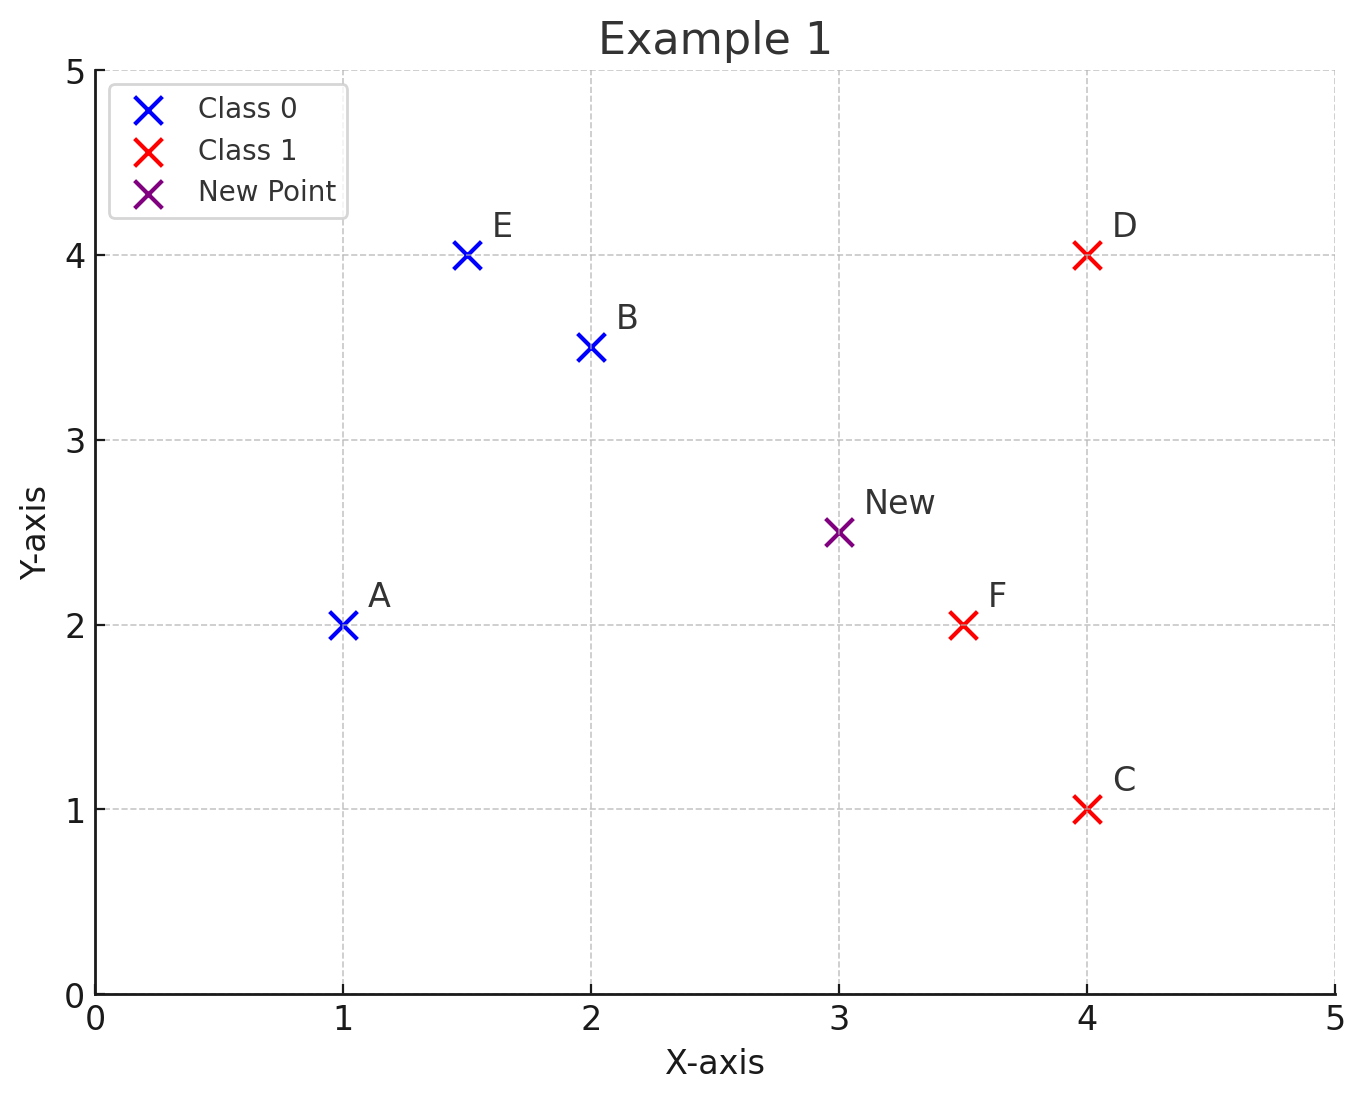
\includegraphics[width=\linewidth]{img/lecture2/example1.png}
% \end{minipage}

% \noindent \textbf{Step 1: Calculate Euclidean Distances}

% \begin{itemize}
%     \item \( d(\text{New Point}, A) = \sqrt{(3 - 1)^2 + (2.5 - 2)^2} = \sqrt{2^2 + 0.5^2} = \sqrt{4.25} \approx 2.06 \)
%     \item \( d(\text{New Point}, B) = \sqrt{(3 - 2)^2 + (2.5 - 3.5)^2} = \sqrt{1^2 + (-1)^2} = \sqrt{2} \approx 1.41 \)
%     \item \( d(\text{New Point}, C) = \sqrt{(3 - 4)^2 + (2.5 - 1)^2} = \sqrt{(-1)^2 + 1.5^2} = \sqrt{3.25} \approx 1.80 \)
%     \item \( d(\text{New Point}, D) = \sqrt{(3 - 4)^2 + (2.5 - 4)^2} = \sqrt{(-1)^2 + (-1.5)^2} = \sqrt{3.25} \approx 1.80 \)
%     \item \( d(\text{New Point}, E) = \sqrt{(3 - 1.5)^2 + (2.5 - 4)^2} = \sqrt{1.5^2 + (-1.5)^2} = \sqrt{4.5} \approx 2.12 \)
%     \item \( d(\text{New Point}, F) = \sqrt{(3 - 3.5)^2 + (2.5 - 2)^2} = \sqrt{(-0.5)^2 + 0.5^2} = \sqrt{0.5} \approx 0.71 \)
% \end{itemize}

% \noindent \textbf{Step 2: Identify Nearest Neighbors}

% \noindent For \( k = 3 \), the nearest neighbors are:
% \begin{itemize}
%     \item Points F, B, and C (tie with D; choose C by index order), since these have the smallest distances.
% \end{itemize}

% \noindent \textbf{Step 3: Assign Class Label}

% \noindent The majority class among the nearest neighbors is:
% \begin{itemize}
%     \item 2 neighbors from Class 1 (F and C), 1 from Class 0 (B). \textbf{Class 1 is assigned}.
% \end{itemize}

% \subsection{Example 2: Classification with an Outlier Using Manhattan Distance}

% \noindent Consider a dataset with an outlier, appearing to be misclassified or on the wrong side of the decision boundary:

% \begin{minipage}{0.4\textwidth}
% \begin{itemize}
%     \item Data Point A: \( (1.2, 2.8) \) - Class 0
%     \item Data Point B: \( (3.7, 4.1) \) - Class 0
%     \item Data Point C: \( (6.2, 5.0) \) - Class 1
%     \item Data Point D: \( (7.5, 3.8) \) - Class 1
%     \item Data Point E: \( (7.2, 4.7) \) - Class 0 \\ (Outlier)
% \end{itemize}
% \noindent The new data point to classify is \( (7.5, 4.5) \) (we'll call it F).
% \end{minipage}
% \begin{minipage}{0.5\textwidth}\raggedleft
% 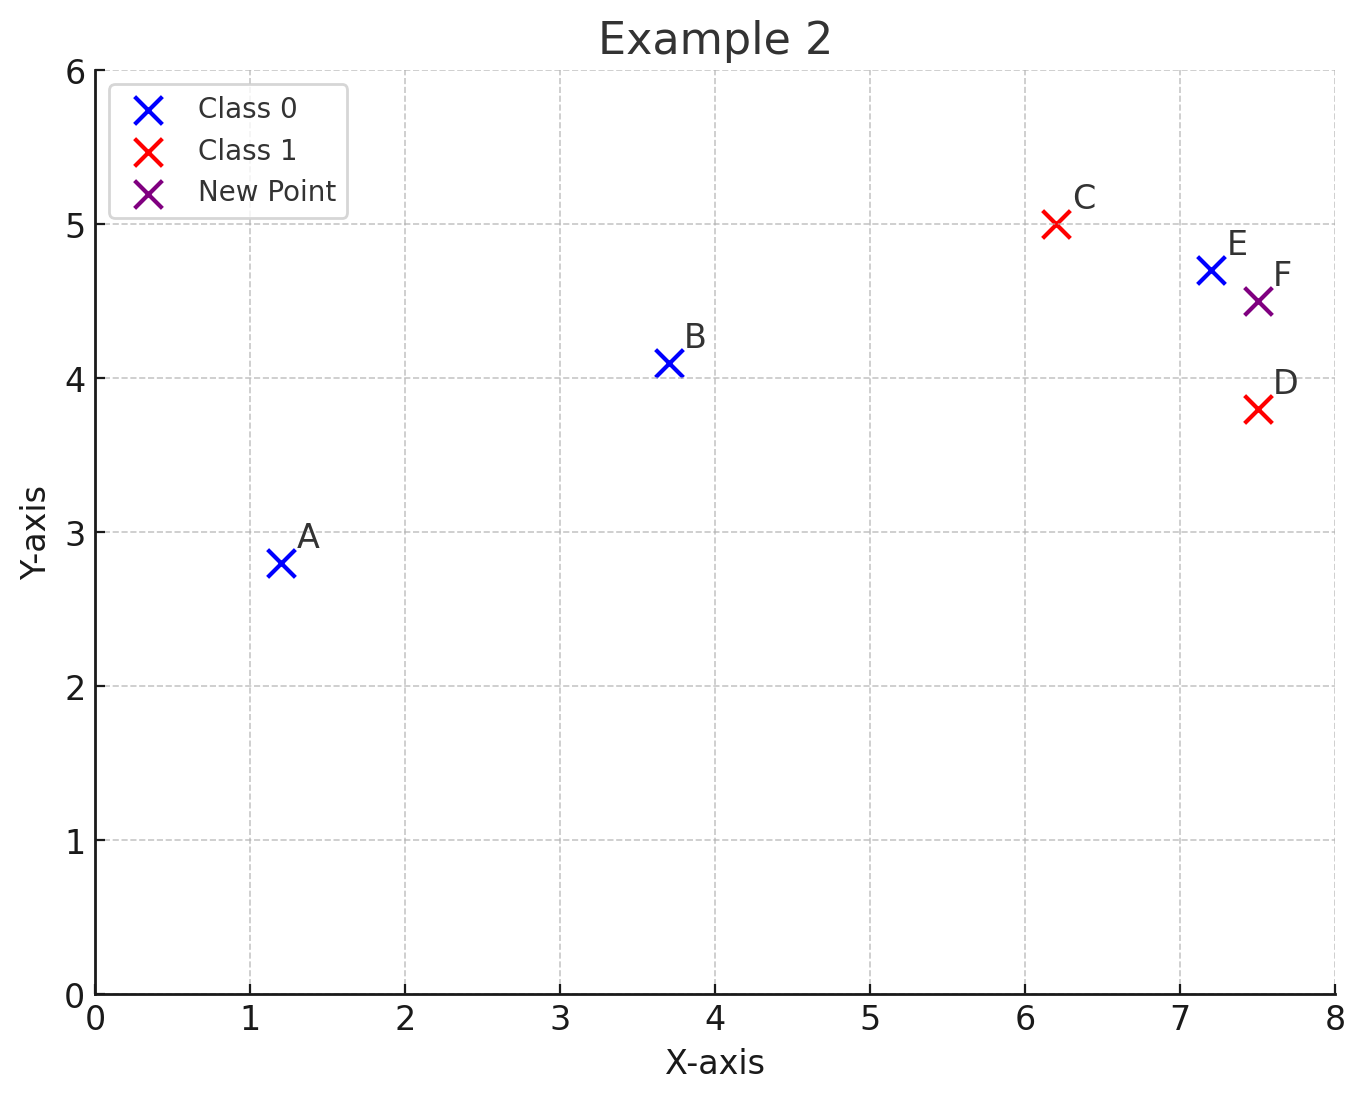
\includegraphics[width=\linewidth]{img/lecture2/example2.png}
% \end{minipage}

% \noindent \textbf{Step 1: Calculate Manhattan Distances}

% \begin{itemize}
%     \item \( d(\text{New Point}, A) = |7.5 - 1.2| + |4.5 - 2.8| = 6.3 + 1.7 = 8.0 \)
%     \item \( d(\text{New Point}, B) = |7.5 - 3.7| + |4.5 - 4.1| = 3.8 + 0.4 = 4.2 \)
%     \item \( d(\text{New Point}, C) = |7.5 - 6.2| + |4.5 - 5.0| = 1.3 + 0.5 = 1.8 \)
%     \item \( d(\text{New Point}, D) = |7.5 - 7.5| + |4.5 - 3.8| = 0.0 + 0.7 = 0.7 \)
%     \item \( d(\text{New Point}, E) = |7.5 - 7.2| + |4.5 - 4.7| = 0.3 + 0.2 = 0.5 \)
% \end{itemize}

% \noindent \textbf{Scenario 1: k = 1, Including Outlier}

% \noindent With \( k = 1 \) and the outlier included, the nearest neighbor is:

% \begin{itemize}
%     \item Point E (the outlier), which is closest with a distance of 0.5.
% \end{itemize}

% \noindent Since Point E is labeled as Class 0, the new point is \textbf{classified as Class 0}.

% \noindent \textbf{Scenario 2: k = 1, Removing Outlier}

% \noindent If we remove the outlier (Point E), the new nearest neighbor is:

% \begin{itemize}
%     \item Point D, with a distance of 0.7.
% \end{itemize}

% \noindent Since Point D is labeled as Class 1, the new point is \textbf{classified as Class 1}.

% \noindent \textbf{Scenario 3: k = 3, Including Outlier}

% \noindent With \( k = 3 \) and the outlier included, the three nearest neighbors are:

% \begin{itemize}
%     \item Point E (Class 0) with a distance of 0.5
%     \item Point D (Class 1) with a distance of 0.7
%     \item Point C (Class 1) with a distance of 1.8
% \end{itemize}

% \noindent The majority class among these neighbors is Class 1 (2 neighbors from Class 1 and 1 from Class 0), so the new point is \textbf{classified as Class 1}.

% Here we see how having outliers, e.g. due to noisy data, can affect the k-NN algorithm. We can see from this example that increasing $k$ made the model less sensitive to the outlier, but if we were to increase $k$ too much then it could lead to underfitting (see below).


% \subsection{Choosing the Value of \( k \)}
% \begin{itemize}
%     \item Selecting \( k \) is crucial:
%     \begin{itemize}
%         \item Small \( k \) values lead to high variance (overfitting).
%         \item Larger \( k \) values reduce variance but can introduce bias (underfitting).
%     \end{itemize}
%     \item Cross-validation can be used to determine the optimal \( k \) by evaluating performance on validation sets.
% \end{itemize}

% \subsection{Feature Scaling}

% \subsubsection{Min-Max Normalization}

% \begin{itemize}
%     \item Distance metrics can be biased if features have different scales.
%     \item For example, in the scenario covered in class, loan amounts (in dollars) may dominate the distance calculation compared to age (in years).
%     \item To address this, features should be normalized:
%     \[
%     x'_{i,j} = \frac{x_{i,j} - \min(x_{:,j})}{\max(x_{:,j}) - \min(x_{:,j})}
%     \]
% \end{itemize}

% Where:
% \begin{itemize}
%     \item \( x'_{i,j} \) is the normalized value of the feature.
%     \item \( x_{i,j} \) is the original value of the feature.
%     \item \( \min(x_{:,j}) \) and \( \max(x_{:,j}) \) are the minimum and maximum values of the feature across the dataset.
% \end{itemize}

% Here we use \textbf{min–max normalization} (scales to [0, 1]). This transformation scales all features to a [0, 1] range, preventing any single feature from dominating the distance computation.

% \subsubsection{Z-Score Standardization}

% \begin{itemize}
%     \item Another common feature scaling method is \textbf{z-score standardization}, which centers the data to mean 0 and scales it to unit variance.
%     \item Useful when features have different spreads/variances and when outliers may affect min–max scaling.
%     \[
%     x'_{i,j} = \frac{x_{i,j} - \mu_j}{\sigma_j}
%     \]
% \end{itemize}

% Where:
% \begin{itemize}
%     \item \( x'_{i,j} \) is the standardized value of feature $j$ for sample $i$.
%     \item \( \mu_j \) is the mean of feature $j$ across the dataset.
%     \item \( \sigma_j \) is the standard deviation of feature $j$ across the dataset.
% \end{itemize}

% Z-score standardization ensures features have comparable scale (mean 0, variance 1), which improves distance-based methods like $k$-NN.

\section{k-Nearest Neighbor (k-NN) Classifier}

The \(k\)-Nearest Neighbor (k-NN) classifier is one of the simplest and most intuitive machine learning algorithms. It is a non-parametric learning method that can be used for both classification and regression tasks. The main idea behind k-NN is that similar data points tend to belong to the same class. Instead of learning an explicit model during training, k-NN makes predictions by directly comparing new data points to previously seen examples.

One of the main strengths of k-NN is its simplicity. The algorithm does not require an explicit training phase in the traditional sense. Instead, it stores the training dataset and performs computation only when a prediction is needed. Because of this, k-NN is sometimes computationally cheap during training but more expensive during prediction, since distances must be computed against many stored samples.

\subsection{Overview}

The k-NN classifier is often described as a \textbf{lazy learner}. This means that, unlike many other machine learning methods, it does not build a compressed model representation during training. Instead, it postpones all computation until a query is made. When a new data point arrives, the algorithm compares it to the stored training data and determines its class based on similarity.

Historically, k-NN dates back to the 1970s and has been widely used in pattern recognition, statistical estimation, and information retrieval. Despite its simplicity, it remains an important baseline method and is often used when interpretability and simplicity are desired.

k-NN is also considered a \textbf{non-parametric} method because it does not assume a fixed functional form for the model. The main parameter that must be chosen is \(k\), the number of neighbors used to make predictions. This flexibility allows the method to adapt to many different data distributions, although it also makes the choice of \(k\) an important design decision.

\subsection{Algorithm}

The basic procedure of the k-NN algorithm can be understood as a sequence of intuitive steps. Suppose we are given a dataset of labeled samples and we want to classify a new data point.

First, we compute the distance between the new sample and every stored sample in the dataset using a chosen distance metric. This step measures how similar the new example is to previously observed examples.

Next, we identify the \(k\) samples that are closest to the new point. These are called the nearest neighbors. The assumption is that these nearby points provide the most useful information about the likely class of the new example.

Finally, we assign the class label based on the majority class among these neighbors. In other words, the new data point is classified according to the most common label among its nearest neighbors.

A useful special case occurs when \(k=1\). In this case, the new sample is simply assigned the class of its single nearest neighbor. While this can lead to very flexible decision boundaries, it can also make the model highly sensitive to noise, resulting in high variance.

\subsection{Distance Metrics}

A key component of k-NN is how distance is measured between data points. Since the algorithm relies entirely on similarity comparisons, the choice of distance metric can strongly influence performance. Let $\mathbf{x}, \mathbf{y} \in \mathbb{R}^d$, where $d$ is the number of features.

One of the most commonly used distance measures is the \textbf{Euclidean distance}, defined as

\[
d(\mathbf{x}, \mathbf{y}) = \sqrt{\sum_{i=1}^{d} (x_i - y_i)^2}.
\]

This distance measures the straight-line distance between two points in feature space. It is most appropriate when features are continuous and have similar scales. However, Euclidean distance can be sensitive to features with large magnitudes.

Another commonly used metric is the \textbf{Manhattan distance}, defined as

\[
d(\mathbf{x}, \mathbf{y}) = \sum_{i=1}^{d} |x_i - y_i|.
\]

This distance measures the sum of absolute differences between feature values. It can be interpreted as the distance traveled along axis-aligned paths (like navigating city blocks). Manhattan distance is sometimes more robust to outliers than Euclidean distance.

A more general formulation is the \textbf{Minkowski distance},

\[
d(\mathbf{x}, \mathbf{y}) =
\left(
\sum_{i=1}^{d} |x_i - y_i|^q
\right)^{\frac{1}{q}},
\]

where $q \geq 1$ is a parameter. This distance generalizes both Euclidean distance (when \(q=2\)) and Manhattan distance (when \(q=1\)). By adjusting \(q\), we can control how strongly large feature differences are penalized.

Finally, when working with categorical data rather than numerical features, the \textbf{Hamming distance} is often used:

\[
d(\mathbf{x}, \mathbf{y}) =
\sum_{i=1}^{d} \mathbf{1}[x_i \neq y_i].
\]

This distance simply counts the number of positions where two feature vectors differ. It is particularly useful for binary features, categorical attributes, or string comparisons.

\subsection{Example 1: Classification Using Euclidean Distance}

To better understand how k-NN works, consider the following example. Suppose we have a dataset consisting of six labeled data points, and we want to classify a new point based on its nearest neighbors.

\begin{minipage}{0.4\textwidth}
\begin{itemize}
    \item Data Point A: \( (1, 2) \) - Class 0
    \item Data Point B: \( (2, 3.5) \) - Class 0
    \item Data Point C: \( (4, 1) \) - Class 1
    \item Data Point D: \( (4, 4) \) - Class 1
    \item Data Point E: \( (1.5, 4) \) - Class 0
    \item Data Point F: \( (3.5, 2) \) - Class 1
\end{itemize}

The new data point to classify is \( (3, 2.5) \).
\end{minipage}
\begin{minipage}{0.5\textwidth}\raggedleft
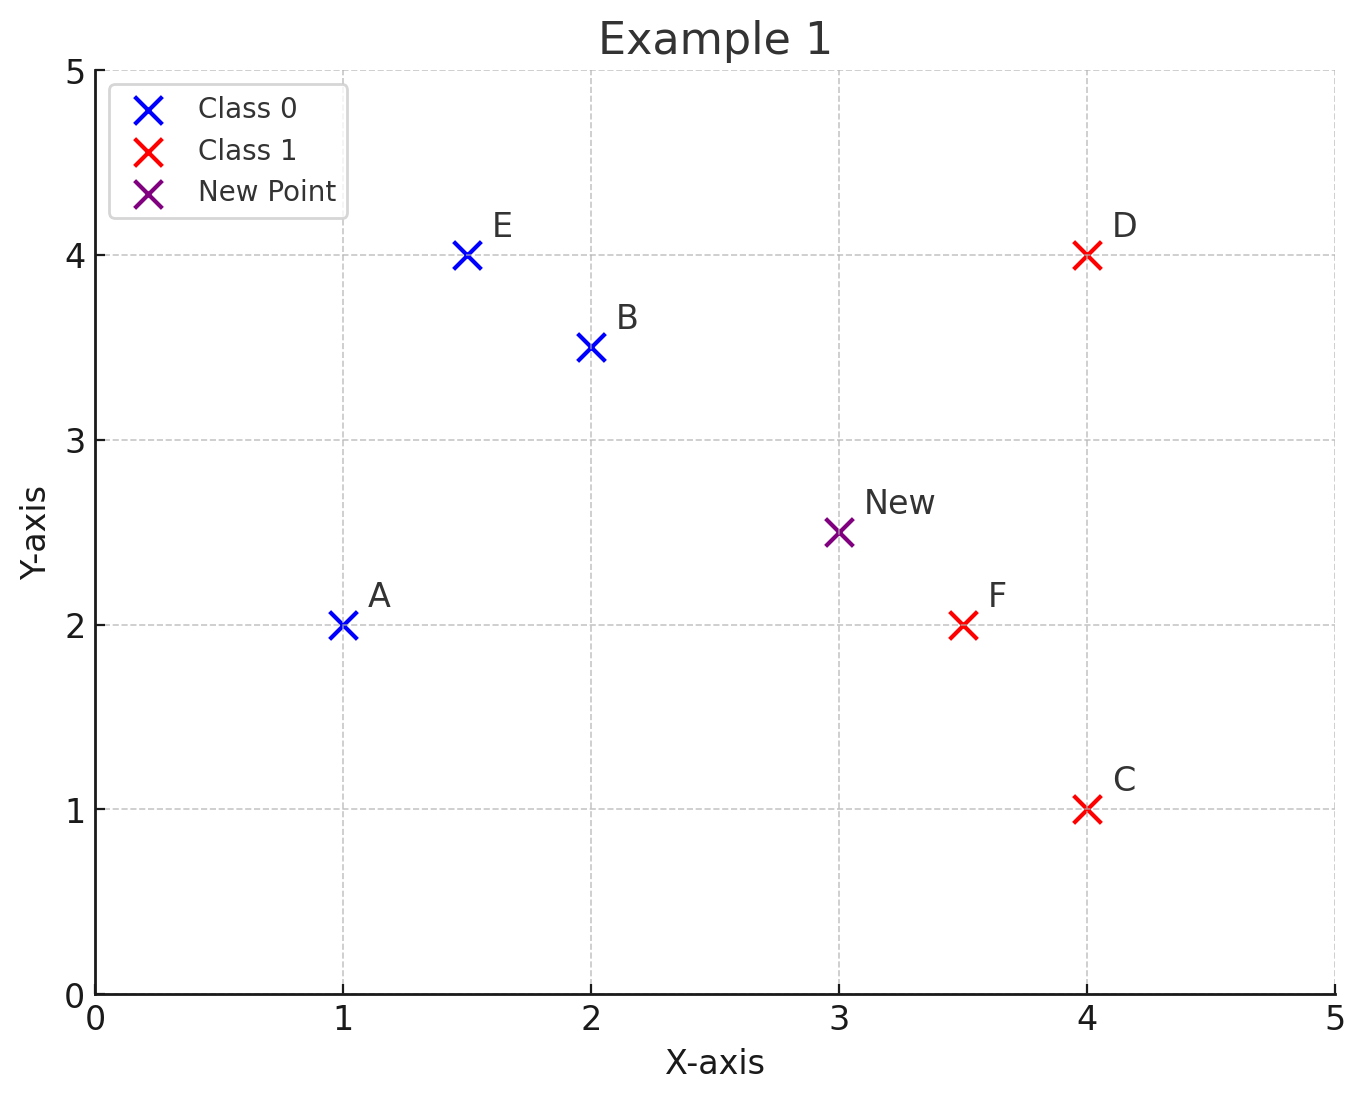
\includegraphics[width=\linewidth]{img/lecture2/example1.png}
\end{minipage}

The first step is to compute the Euclidean distance between the new point and each existing point.

\textbf{Step 1: Calculate Euclidean Distances}

\begin{itemize}
    \item \( d(\text{New Point}, A) \approx 2.06 \)
    \item \( d(\text{New Point}, B) \approx 1.41 \)
    \item \( d(\text{New Point}, C) \approx 1.80 \)
    \item \( d(\text{New Point}, D) \approx 1.80 \)
    \item \( d(\text{New Point}, E) \approx 2.12 \)
    \item \( d(\text{New Point}, F) \approx 0.71 \)
\end{itemize}

Next, we identify the nearest neighbors.

\textbf{Step 2: Identify Nearest Neighbors}

If we choose \(k=3\), the three closest points are F, B, and C (with C chosen over D in the tie). These points therefore determine the prediction.

\textbf{Step 3: Assign Class Label}

Among these neighbors, two belong to Class 1 (F and C) and one belongs to Class 0 (B). Since Class 1 is the majority, the new point is classified as \textbf{Class 1}.

\subsection{Example 2: Classification with an Outlier Using Manhattan Distance}

Now consider a second example where an outlier is present in the dataset.

\begin{minipage}{0.4\textwidth}
\begin{itemize}
    \item Data Point A: \( (1.2, 2.8) \) - Class 0
    \item Data Point B: \( (3.7, 4.1) \) - Class 0
    \item Data Point C: \( (6.2, 5.0) \) - Class 1
    \item Data Point D: \( (7.5, 3.8) \) - Class 1
    \item Data Point E: \( (7.2, 4.7) \) - Class 0 (Outlier)
\end{itemize}

The new data point to classify is \( (7.5, 4.5) \).
\end{minipage}
\begin{minipage}{0.5\textwidth}\raggedleft
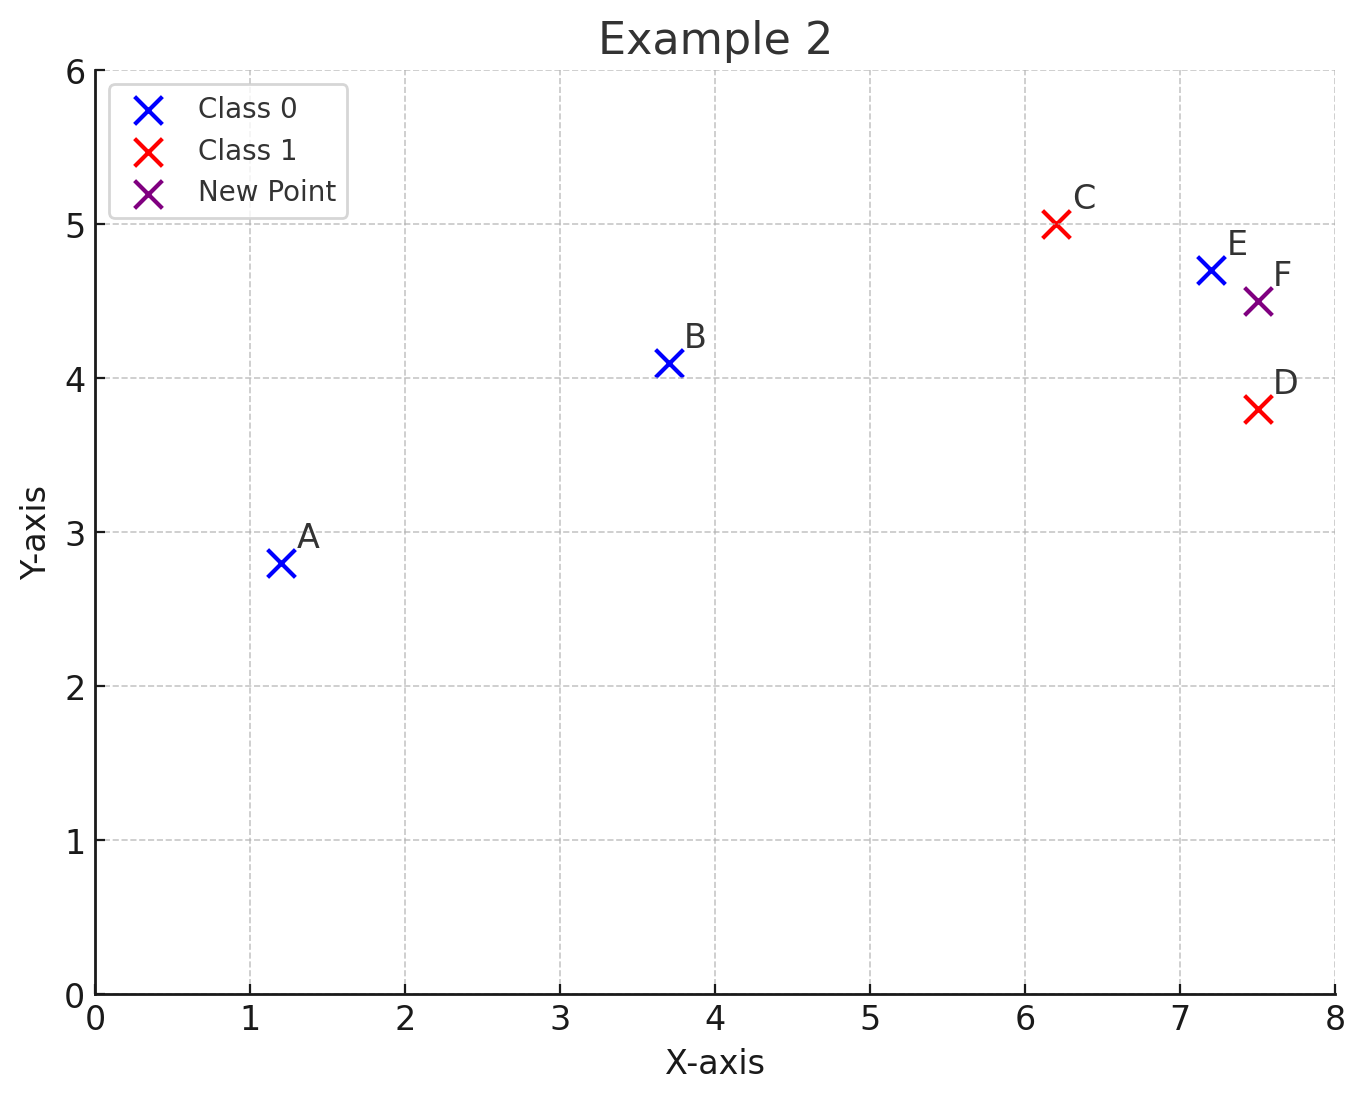
\includegraphics[width=\linewidth]{img/lecture2/example2.png}
\end{minipage}

After computing Manhattan distances, we can examine how the choice of \(k\) affects robustness to the outlier.

When \(k=1\), the closest point is the outlier (Point E), so the new point is classified as Class 0. However, if we remove the outlier, the nearest neighbor becomes Point D, resulting in a Class 1 prediction.

If instead we use \(k=3\), the three nearest neighbors include two Class 1 points and one Class 0 point. This leads to a Class 1 prediction, showing how larger values of \(k\) can reduce sensitivity to noise.

This example illustrates an important tradeoff. Small values of \(k\) can lead to very flexible decision boundaries but may be sensitive to noise. Larger values of \(k\) provide smoother decision boundaries but may oversimplify the data structure.

\subsection{Choosing the Value of \(k\)}

Choosing the value of \(k\) is one of the most important design decisions in k-NN. Small values of \(k\) tend to produce models with low bias but high variance, meaning they may overfit the training data. Larger values of \(k\) reduce variance but may increase bias, potentially causing underfitting.

In practice, cross-validation is commonly used to determine a good value of \(k\). By evaluating performance on validation data, we can select a value that balances bias and variance appropriately.

\subsection{Feature Scaling}

Because k-NN relies on distance calculations, it is very sensitive to the scale of features. If one feature has values much larger than another, it may dominate the distance calculation even if it is not more important.

\subsubsection{Min-Max Normalization}

One common solution is \textbf{min–max normalization}, which rescales each feature to lie between 0 and 1:

\[
x'_{i,j} =
\frac{x_{i,j} - \min(x_{:,j})}
{\max(x_{:,j}) - \min(x_{:,j})}.
\]

Here, \(x'_{i,j}\) represents the normalized value, while \(\min(x_{:,j})\) and \(\max(x_{:,j})\) represent the minimum and maximum values of the feature across the dataset. This transformation ensures that all features contribute more equally to distance calculations.

\subsubsection{Z-Score Standardization}

Another widely used scaling method is \textbf{z-score standardization}, which transforms features to have mean zero and unit variance:

\[
x'_{i,j} =
\frac{x_{i,j} - \mu_j}{\sigma_j}.
\]

Here, \(\mu_j\) is the mean of feature \(j\), and \(\sigma_j\) is its standard deviation. This method is particularly useful when features have different variances or when outliers may distort min–max scaling.

By ensuring that features are on comparable scales, these normalization techniques significantly improve the performance and reliability of distance-based methods such as k-NN.

\section{Na\"ive Bayes Classifier}

The Na\"ive Bayes classifier is a probabilistic classification method based on Bayes' theorem. Its defining assumption is that the input features are \textit{conditionally independent} given the class label. This assumption is called ``na\"ive'' because, in many real-world datasets, features are not truly independent. Nevertheless, the method often performs surprisingly well in practice, especially in applications such as text classification, spam filtering, and document categorization.

One reason Na\"ive Bayes is so useful is that it provides a simple and mathematically interpretable way to estimate the probability of each class for a given input. Rather than directly learning a decision boundary as some classifiers do, it models how likely the observed features are under each class and then uses probability rules to infer the most likely class. This makes it a natural example of a probabilistic classifier.

\subsection{Overview}

The central assumption of the Na\"ive Bayes classifier is that all features are conditionally independent once the class label is known. In other words, after conditioning on the class, the value of one feature is assumed not to affect the value of another. Although this assumption is often not exactly true, it greatly simplifies both the mathematics and the estimation procedure.

Na\"ive Bayes is also a \textbf{generative model}. This means it models the class prior \(P(y)\) and the class-conditional distribution \(P(\mathbf{x}\mid y)\), rather than directly modeling \(P(y\mid \mathbf{x})\). Once these quantities are estimated, Bayes' theorem is used to compute the posterior probability of each class given the observed feature vector. Because it only requires estimating relatively simple probabilities or feature statistics, Na\"ive Bayes is especially effective when the data is high-dimensional or when only a modest amount of training data is available.

\subsection{Bayes' Theorem}

The Na\"ive Bayes classifier is built on Bayes' theorem:
\[
P(y \mid \mathbf{x}) = \frac{P(\mathbf{x} \mid y)P(y)}{P(\mathbf{x})}.
\]

This equation relates several important probabilities. The term \(P(y \mid \mathbf{x})\) is called the \textbf{posterior probability}; it is the probability that the class is \(y\) after observing the feature vector \(\mathbf{x}\). The term \(P(\mathbf{x} \mid y)\) is called the \textbf{likelihood}; it measures how likely the observed feature vector is under class \(y\). The term \(P(y)\) is the \textbf{prior probability} of class \(y\), reflecting how common that class is before seeing the input. Finally, \(P(\mathbf{x})\) is the \textbf{evidence} or marginal likelihood, which ensures that the posterior probabilities across all classes sum to one.

When making a prediction, \(P(\mathbf{x})\) is the same for all candidate classes because the observed feature vector is fixed. Therefore, for classification purposes, we often compare classes using the proportional relation
\[
P(y \mid \mathbf{x}) \propto P(\mathbf{x} \mid y)P(y).
\]

The ``na\"ive'' assumption now enters the picture. If we assume that the features \(x_1, x_2, \dots, x_d\) are conditionally independent given the class label \(y\), then the likelihood can be factorized as
\[
P(\mathbf{x} \mid y) = \prod_{i=1}^{d} P(x_i \mid y).
\]

This simplification is what makes Na\"ive Bayes computationally attractive. Instead of estimating a potentially very complicated joint distribution over all features, we only need to estimate one-feature-at-a-time conditional probabilities. As a result, the posterior used for prediction becomes
\[
P(y \mid \mathbf{x}) \propto P(y)\prod_{i=1}^{d} P(x_i \mid y).
\]

Even though the independence assumption is strong and often violated in real datasets, Na\"ive Bayes can still perform well because correct classification does not require the estimated probabilities to be perfect. In many problems, it is enough for the model to rank the candidate classes correctly.

\subsection{Types of Na\"ive Bayes Models}

There are several variants of Na\"ive Bayes, and the appropriate version depends on the nature of the feature values.

\textbf{Gaussian Na\"ive Bayes} is used when the features are continuous-valued. In this model, each feature is assumed to follow a Gaussian (normal) distribution within each class. For each class \(y\), the model estimates a mean and variance for each feature using the training examples that belong to that class. The conditional likelihood of feature \(x_i\) under class \(y\) is then given by
\[
P(x_i \mid y) =
\frac{1}{\sqrt{2\pi\sigma_y^2}}
\mathrm{e}^{-\frac{(x_i - \mu_y)^2}{2\sigma_y^2}}.
\]
Under the Na\"ive Bayes assumption, the full likelihood becomes
\[
P(\mathbf{x} \mid y) = \prod_{i=1}^{d} P(x_i \mid y).
\]
In practice, the mean and variance are usually estimated separately for each feature and each class. Gaussian Na\"ive Bayes is a good fit when the data consists of real-valued measurements such as lengths, temperatures, or sensor values.

\textbf{Multinomial Na\"ive Bayes} is commonly used for count-based data, especially in text classification. In document modeling, for example, the features may represent how many times each word appears in a document. In this setting, the likelihood is modeled using a multinomial distribution:
\[
P(\mathbf{x} \mid y)=
\frac{\left(\sum_{j=1}^d x_j\right)!}{\prod_{j=1}^d x_j!}
\prod_{j=1}^d \theta_{y,j}^{\,x_j}.
\]
Here, \(\theta_{y,j}\) denotes the probability of feature \(j\) under class \(y\). The multinomial coefficient is constant with respect to the class and is therefore often omitted during classification, since it does not affect which class receives the highest posterior score. Multinomial Na\"ive Bayes is especially popular in bag-of-words models for text.

\textbf{Bernoulli Na\"ive Bayes} is used when the features are binary indicators. In this case, each feature simply records whether a certain attribute is present or absent. For instance, in spam filtering, a feature might indicate whether the word ``free'' appears in an email. If \(x_j \in \{0,1\}\), then the likelihood under class \(y\) is
\[
P(\mathbf{x} \mid y)=\prod_{j=1}^d p_{y,j}^{\,x_j}(1-p_{y,j})^{(1-x_j)}.
\]
This model is well-suited for feature vectors that describe presence or absence rather than counts or continuous measurements.

\subsection{Advantages and Disadvantages}

Na\"ive Bayes has several practical advantages. First, it is computationally efficient. Training is usually fast because the model only needs to estimate simple quantities such as counts, means, variances, or conditional probabilities. Prediction is also fast, which makes the method suitable for large datasets and real-time applications.

A second advantage is that Na\"ive Bayes naturally handles multi-class problems. Unlike some classifiers that are fundamentally binary and require additional design choices to extend to multiple classes, Na\"ive Bayes directly computes posterior scores for each class and selects the most probable one.

A third advantage is its low storage requirement. Rather than storing all training examples, as in case-based methods like k-NN, Na\"ive Bayes only stores a small number of parameters per class. This can make it memory-efficient and easy to deploy.

However, Na\"ive Bayes also has important limitations. One well-known issue is the \textbf{zero-frequency problem}. If a certain feature value never appears with a particular class in the training data, then the estimated conditional probability for that event becomes zero. Because Na\"ive Bayes multiplies many such probabilities together, a single zero can force the entire posterior score for that class to zero. This problem is often addressed by smoothing techniques such as Laplace smoothing.

Another limitation is the strong independence assumption. In many real-world datasets, features are correlated. For example, in text data, the presence of one word may make another word more likely to appear. Since Na\"ive Bayes ignores such dependencies, its estimated probabilities may not accurately reflect the true underlying distribution.

Finally, Na\"ive Bayes is often criticized for poor probability calibration. Even when it predicts the correct class, the numerical probabilities it produces may be overly confident. This means that while it can be an excellent classifier, its posterior probabilities should not always be interpreted as highly accurate confidence estimates.

\subsection{Applications}

Na\"ive Bayes is widely used in text classification tasks such as spam detection, sentiment analysis, topic labeling, and document categorization. It is especially effective in these settings because text data often has very high dimensionality, and the method can still train efficiently with relatively limited data.

The model is also suitable for real-time prediction tasks because of its low computational cost. Once the necessary probabilities or statistics have been estimated, prediction can be performed very quickly.

In addition, Na\"ive Bayes has been used in recommendation-related and content-based filtering settings, where classes or preferences may be inferred from observed item or user attributes. While more sophisticated models are often used in large-scale recommendation systems, Na\"ive Bayes provides a useful and interpretable baseline.

\subsection{Example (done in class \& available in lecture slides)}

Consider a weather dataset in which the goal is to predict whether a game will be played based on observed weather conditions such as whether it is sunny or rainy, and whether the wind is strong or weak. A Na\"ive Bayes solution to this problem typically begins by converting the dataset into a set of frequency counts. These counts are then used to estimate the likelihood of each feature value under each class. Finally, Bayes' theorem is applied to compute the posterior probability for each class, and the class with the larger posterior probability is chosen as the prediction.

This general workflow appears repeatedly in Na\"ive Bayes applications: first estimate priors and class-conditional probabilities from data, then combine them probabilistically to classify new inputs.

\subsection{Another Example: Email Spam Classification}

In this example, we build a simple spam filter using the Bernoulli Na\"ive Bayes classifier. The goal is to classify emails as either ``Spam'' or ``Not Spam'' based on whether certain keywords are present.

\noindent \textbf{Step 1: Dataset}

Consider the following dataset of emails. Each feature indicates whether a specific keyword is present (1) or absent (0).

\begin{center}
\begin{tabular}{|c|c|c|c|c|}
\hline
\textbf{Email} & \textbf{Contains ``offer"} & \textbf{Contains ``free"} & \textbf{Contains ``win"} & \textbf{Class} \\
\hline
1 & 1 & 1 & 1 & Spam \\
2 & 1 & 0 & 1 & Spam \\
3 & 0 & 1 & 1 & Spam \\
4 & 0 & 1 & 0 & Not Spam \\
5 & 1 & 0 & 0 & Not Spam \\
6 & 0 & 0 & 1 & Spam \\
7 & 0 & 0 & 0 & Not Spam \\
\hline
\end{tabular}
\end{center}

We would like to classify a new email with feature vector \( (1,1,0) \). This means the email contains the words ``offer'' and ``free,'' but does not contain the word ``win.''

\noindent \textbf{Step 2: Convert the Dataset into Frequency Tables}

To apply Na\"ive Bayes, we first count how often each feature value appears within each class.

\medskip
\noindent \textbf{Feature: contains ``offer''}
\begin{center}
\begin{tabular}{|c|cc|c|}
\hline
 & Spam & Not Spam & Total \\
\hline
Yes (1) & 2 & 1 & 3 \\
No (0) & 2 & 2 & 4 \\
\hline
Total & 4 & 3 & 7 \\
\hline
\end{tabular}
\end{center}

\noindent \textbf{Feature: contains ``free''}
\begin{center}
\begin{tabular}{|c|cc|c|}
\hline
 & Spam & Not Spam & Total \\
\hline
Yes (1) & 2 & 1 & 3 \\
No (0) & 2 & 2 & 4 \\
\hline
Total & 4 & 3 & 7 \\
\hline
\end{tabular}
\end{center}

\noindent \textbf{Feature: contains ``win''}
\begin{center}
\begin{tabular}{|c|cc|c|}
\hline
 & Spam & Not Spam & Total \\
\hline
Yes (1) & 4 & 0 & 4 \\
No (0) & 0 & 3 & 3 \\
\hline
Total & 4 & 3 & 7 \\
\hline
\end{tabular}
\end{center}

\noindent \textbf{Step 3: Build the Likelihood Table}

Using these frequency tables, we estimate the conditional probabilities needed for Bernoulli Na\"ive Bayes.

\begin{center}
\begin{tabular}{|c|c|c|}
\hline
\textbf{Feature} & \textbf{P(Feature $\mid$ Spam)} & \textbf{P(Feature $\mid$ Not Spam)} \\
\hline
Contains ``offer'' (1) & \(2/4\) & \(1/3\) \\
Does not contain ``offer'' (0) & \(2/4\) & \(2/3\) \\
\hline
Contains ``free'' (1) & \(2/4\) & \(1/3\) \\
Does not contain ``free'' (0) & \(2/4\) & \(2/3\) \\
\hline
Contains ``win'' (1) & \(4/4\) & \(0/3\) \\
Does not contain ``win'' (0) & \(0/4\) & \(3/3\) \\
\hline
\end{tabular}
\end{center}

\noindent \textbf{Step 4: Apply Bayes' Theorem and Make a Prediction}

We now compute the posterior score for each class. Since the same evidence term appears in both class posteriors, we only need to compare the unnormalized posterior values.

The prior probabilities are
\[
P(\text{Spam}) = \frac{4}{7},
\qquad
P(\text{Not Spam}) = \frac{3}{7}.
\]

For the new email \( (1,1,0) \), the spam score is
\[
P(\text{Spam} \mid (1,1,0))
\propto
P(\text{Spam})
\times
P(\text{offer}=1 \mid \text{Spam})
\times
P(\text{free}=1 \mid \text{Spam})
\times
P(\text{win}=0 \mid \text{Spam}),
\]
so
\[
P(\text{Spam} \mid (1,1,0))
\propto
\frac{4}{7}\times\frac{2}{4}\times\frac{2}{4}\times\frac{0}{4}
= 0.
\]

Similarly, the score for Not Spam is
\[
P(\text{Not Spam} \mid (1,1,0))
\propto
P(\text{Not Spam})
\times
P(\text{offer}=1 \mid \text{Not Spam})
\times
P(\text{free}=1 \mid \text{Not Spam})
\times
P(\text{win}=0 \mid \text{Not Spam}),
\]
which gives
\[
P(\text{Not Spam} \mid (1,1,0))
\propto
\frac{3}{7}\times\frac{1}{3}\times\frac{1}{3}\times\frac{3}{3}
=
\frac{1}{21}.
\]

Since the score for Spam is zero and the score for Not Spam is positive, the classifier predicts that the new email is \textbf{Not Spam}.

This example clearly shows the \textbf{zero-frequency problem}. Because the training set contains no spam emails without the word ``win,'' the model assigns
\[
P(\text{win}=0 \mid \text{Spam}) = 0,
\]
and this single zero causes the entire posterior score for the Spam class to collapse to zero. In practice, this issue is typically handled using \textbf{Laplace smoothing}, which adds a small positive count to each feature-class combination so that no probability becomes exactly zero.

\section{Additional Details}

Before moving further into machine learning, it is useful to clarify several foundational terms that appear throughout this lecture and in many other learning problems.

A \textbf{sample} is a single data item that the model processes. Depending on the application, a sample could be a document, an image, an audio clip, a video segment, a row in a spreadsheet or database, or any other object that can be represented numerically. In machine learning, each sample corresponds to one example in the dataset.

\textbf{Features} are the measurable properties or descriptive attributes used to represent a sample. These may include physical measurements, counts, categories converted into numbers, or other characteristics that capture useful information about the data item. The choice of features is important because it determines what information the model can use to make predictions.

A \textbf{feature vector} is the numerical representation of a sample obtained by combining all of its features into a single vector. If a sample is described by \(n\) features, then its representation is an \(n\)-dimensional vector. This feature vector serves as the input to a machine learning model.

\textbf{Feature extraction} is the process of transforming raw data into a feature vector. In many cases, raw data such as images, audio, or text is not directly suitable for a classical machine learning algorithm, so it must first be converted into a structured numerical representation. Feature extraction may also reduce dimensionality by retaining the most informative aspects of the data while discarding less useful details.

The \textbf{target class} is the correct output label that a model is intended to predict in a classification problem. For example, the target class could indicate the species of a flower, whether an email is spam, or whether an image contains a certain object. In supervised learning, the training data includes these target labels so that the model can learn the relationship between inputs and outputs.

A \textbf{learning model} is the family or class of functions that the algorithm searches over in order to approximate the mapping from inputs to outputs. This includes both the structure of the model and its learnable parameters. For example, a decision tree, a logistic regression classifier, and a neural network are all different kinds of learning models.

The \textbf{training algorithm} is the procedure used to adjust the model parameters based on the training data. Its goal is to improve the model’s performance by finding parameter values that produce accurate predictions. Examples of training algorithms include gradient descent, backpropagation, and other optimization procedures.

Finally, the \textbf{training set} is the portion of the dataset used to fit the model, while the \textbf{evaluation set} (or test set) is used to assess the model’s performance on previously unseen data. This distinction is important because a good machine learning model should not only perform well on the training data, but also generalize well to new examples.

\section{Q\&A Section}

\begin{enumerate}

\item Assume that you are given the Iris dataset, consisting of flower measurements. Recall that each measurement is comprised of four variables, denoted by \([x_1\; x_2\; x_3\; x_4]\). Here \(x_1\) is the sepal length, \(x_2\) is the sepal width, \(x_3\) is the petal length, and \(x_4\) is the petal width. All the measurements are continuous variables in centimeter units. A machine learning model \(f(\cdot)\) is trained to estimate \(x_4\) given \([x_1\; x_2\; x_3]\) as the inputs. Which one of the following tasks does \(f(\cdot)\) perform?

\begin{enumerate}
    \item Classification
    \item Regression
\end{enumerate}

\textbf{Solution:} \\
b) Regression

\textbf{Explanation:} \\
The model \(f(\cdot)\) is predicting a continuous variable \(x_4\) based on other continuous variables \([x_1\; x_2\; x_3]\). Since the output is a real-valued quantity rather than a discrete class label, this is a regression task.

\item \textbf{Question:} \\
You are given a dataset of handwritten digit images. Each image has been labeled with the correct digit (0–9). However, you are asked to develop a system that groups the images based on similarity, without using the provided labels during the training process.

Which type of learning approach should you use for this task?

\begin{enumerate}
    \item Supervised Learning
    \item Unsupervised Learning
\end{enumerate}

\textbf{Solution:} \\
b) Unsupervised Learning

\textbf{Explanation:} \\
Even though the dataset contains labels, the task explicitly states that the labels should not be used during training. Since the goal is to group similar images together based only on their features, this corresponds to unsupervised learning (specifically clustering).

\item Given the following four points in a 2D space:

\[
P_1 = (1,2), \quad P_2 = (3,4), \quad P_3 = (5,1), \quad P_4 = (7,3)
\]

Calculate the \(k=2\) nearest neighbors to the new point \(P_{\text{new}}=(4,2)\) using the Manhattan distance metric.

\textbf{Solution:} \\
\(P_3\) and one of \(\{P_1, P_2\}\)

\textbf{Explanation:} \\
First compute the Manhattan distance between the new point and each existing point:

\[
\text{Distance to } P_1 = |4-1| + |2-2| = 3
\]

\[
\text{Distance to } P_2 = |4-3| + |2-4| = 1+2 = 3
\]

\[
\text{Distance to } P_3 = |4-5| + |2-1| = 1+1 = 2
\]

\[
\text{Distance to } P_4 = |4-7| + |2-3| = 3+1 = 4
\]

The closest point is \(P_3\) with distance 2. The next closest distance is 3, which is shared by both \(P_1\) and \(P_2\). Therefore, the second nearest neighbor is not unique unless a tie-breaking rule is specified. Thus the two nearest neighbors are \(P_3\) and either \(P_1\) or \(P_2\).

\item Given the following feature values for a dataset (feature 1):

\[
\mathbf{x}_{:,1} = [42, 23, 4, 16, 15, 8]
\]

Normalize the data using min–max normalization to scale the feature to the range \([0,1]\). Provide the normalized value for \(x_{4,1}=16\).

\textbf{Solution:} \\
0.316

\textbf{Explanation:} \\
First compute the minimum and maximum values:

\[
\min(\mathbf{x}_{:,1}) = 4, \qquad \max(\mathbf{x}_{:,1}) = 42
\]

Apply the min–max normalization formula:

\[
x_{4,1}' =
\frac{x_{4,1}-\min(\mathbf{x}_{:,1})}
{\max(\mathbf{x}_{:,1})-\min(\mathbf{x}_{:,1})}
=
\frac{16-4}{42-4}
=
\frac{12}{38}
\approx 0.316
\]

Thus, the normalized value of \(x_{4,1}=16\) is approximately 0.316.

\item In a Na\"ive Bayes classifier, you are given the following prior probabilities and likelihoods for two binary features ``free'' and ``win'':

\[
P(\text{Spam}) = 0.5, \qquad P(\text{Not Spam}) = 0.5
\]

\[
P(\text{``free''}=1 \mid \text{Spam}) = 0.6, \qquad
P(\text{``free''}=1 \mid \text{Not Spam}) = 0.3
\]

\[
P(\text{``win''}=1 \mid \text{Spam}) = 0.7, \qquad
P(\text{``win''}=1 \mid \text{Not Spam}) = 0.2
\]

\textbf{(i) Calculate the unnormalized Na\"ive Bayes score for Spam given that the email contains both words.}

\textbf{Solution:} \\
0.21

\textbf{Explanation:} \\
Using the Na\"ive Bayes independence assumption:

\[
P(\text{``free''}=1,\text{``win''}=1 \mid \text{Spam})
=
0.6 \times 0.7
=
0.42.
\]

The unnormalized Na\"ive Bayes score is:

\[
\text{Score}(\text{Spam})
=
P(\text{Spam})
P(\text{``free''}=1 \mid \text{Spam})
P(\text{``win''}=1 \mid \text{Spam})
=
0.5 \times 0.6 \times 0.7
=
0.21.
\]

\textbf{(ii) Compute the normalized posterior probability}

\[
P(\text{Spam}\mid \text{``free''}=1,\text{``win''}=1).
\]

\textbf{Solution:}

\[
P(\text{Spam}\mid x)
=
\frac{0.21}{0.21+0.03}
=
0.875.
\]

\textbf{Explanation:} \\
First compute the unnormalized score for Not Spam:

\[
P(\text{``free''}=1,\text{``win''}=1 \mid \text{Not Spam})
=
0.3 \times 0.2
=
0.06,
\]

\[
\text{Score}(\text{Not Spam})
=
0.06 \times 0.5
=
0.03.
\]

Now normalize:

\[
P(\text{Spam}\mid x)
=
\frac{\text{Score}(\text{Spam})}
{\text{Score}(\text{Spam})+\text{Score}(\text{Not Spam})}
=
\frac{0.21}{0.24}
=
0.875.
\]

\textbf{(iii) Based on your result, classify the email.}

\textbf{Solution:} \\
Spam

\textbf{Explanation:} \\
Since

\[
P(\text{Spam}\mid x)=0.875
>
P(\text{Not Spam}\mid x)=0.125,
\]

the classifier predicts the email is \textbf{Spam}.

\end{enumerate}

\end{document}